\subsection{Forward modelling}
To illustrate the DC resistivity forward modelling algorithm, we generate synthetic data that would be acquired over the 2D conductivity structure shown in Figure \ref{fig:fwdTrue}. The model region consists of a 10 meter thick overburden having conductivity of 0.1 mS/m on the left and 2 mS/m on the right. A V-shaped valley is cut out to simulate the surface topography. Two conductors are buried in the underlying background of 1 mS/m. On the left, a dipping conductor having a dip of 135$^/circ$ and conductivity of 100 mS/m is buried at a depth of 20 m to the top. On the right, a 50 meter long, 20 meter thick conductive block of 100 mS/m is buried at a depth of 25 meters. Rather than keep the model as discrete blocks we have attempted to make it more geologically realistic by applying a smoothing filter to the model. The model is divided into 48 cells in the $x-$direction and 27 cells in the $z-$direction including a total of 1296 cells. The finite difference mesh is shown in Figure \ref{fig:fwdMsh}. In the survey, surface electrodes are located every ten meters in the interval $x = (-100, 100)$ meters. We compute the potential differences from a pole-dipole array with the potential electrodes on the right. Our designation for this is \textit{PDR} (Potential Dipole Right). There are 19 possible current electrode locations and we record the data for each electrode to a maximum $n-$spacing of 8. The observed data set consists of 124 potential difference values. It is our intention to use these data as input to an inversion. In order to make them more realistic we contaminate each datum by adding Gaussian noise having a standard deviation equal to 5\% of the true potential. The apparent resistivity pseudo-section is shown in Figure \ref{fig:fwdAR}. That figure can be compared with the conductivity model within the region of interest in Figure \ref{fig:fwdTrueCrop}. There is some manifestation of the horizontal conductive block, but much of the conducting ``pants leg'' anomaly seen is really the result of the near surface variation of conductivity and topography. 
%
\begin{figure}
\centering
\subfloat[][]{\label{fig:fwdTrue} 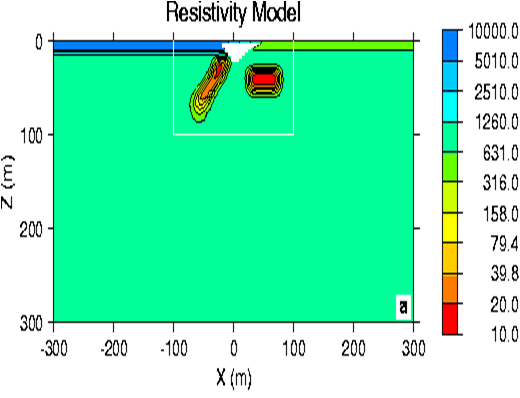
\includegraphics[width=0.5\columnwidth]{fwdTrue}} \\ 
\subfloat[][]{\label{fig:fwdMsh}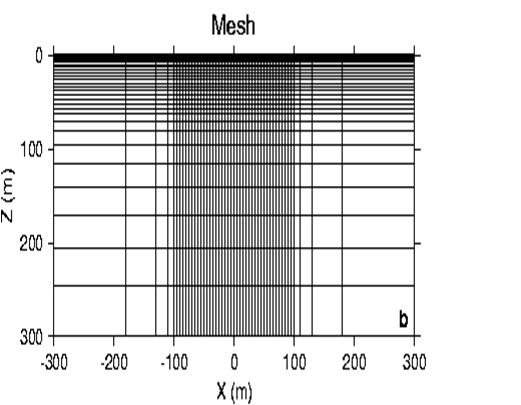
\includegraphics[width=0.5\columnwidth]{fwdMesh}}
\caption{(a) The synthetic model consists of two conductors buried in a uniform halfspace overlain by an overburden of variable conductivity. A V-shaped valley simulates the surface topography. The region of interest is outlined by the white lines, but padding cells are added so that the correct boundary conditions can be applied during the forward modelling. (b) The finite-difference mesh used in the modelling.}
\end{figure}
%
\begin{figure}
\centering
\subfloat[][]{\label{fig:fwdAR} 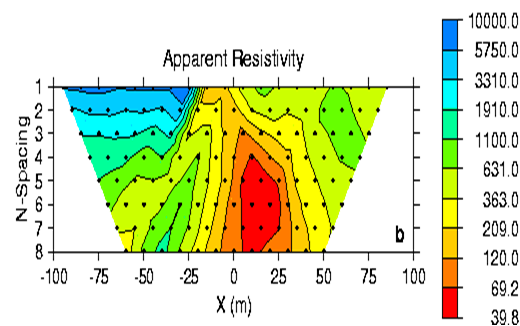
\includegraphics[width=0.5\columnwidth]{fwdAppRes}} \\ 
\subfloat[][]{\label{fig:fwdTrueCrop}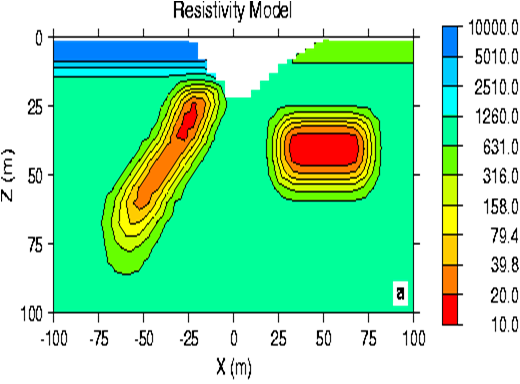
\includegraphics[width=0.5\columnwidth]{fwdTrueCropped}}
\caption{(a) The conductivity model, which is the same as the region outlined in Figure \ref{fig:fwdTrue}. (b) The apparent resistivity pseudo-section measured using a pole-dipole array with $a=10$ m and $n=1,8$. The data have been contaminated by Gaussian noise.}
\end{figure}

The forward modelling for the IP data is also performed with the program \codeName{DCIPF2D}. To calculate IP data, the program performs two DC forward modelling routines and the IP data are generated by the operations indicated in equation \ref{eq:genApChargeDC}. For a synthetic example, we choose the chargeability model in Figure \ref{fig:fwdTrueCharge}. It consists of a chargeable layer at the surface with  $\eta = 0.05$ and two chargeable blocks of $\eta = 0.15$ at depth. The 124 IP data collected in the survey are also contaminated with Gaussian noise having a standard deviation equal to 5\% of the accurate value of the apparent chargeabilites, plus an additional floor of 0.001. The apparent chargeabilities are plotted as percentages in pseudo-section form in Figure \ref{fig:fwdAppCharge}. There is little manifestation of the chargeable block, which is the target for this inversion, but the user is faced with the difficulty of deciding how much of the high chargeability feature sloping downward to the left is the result of a pant leg from the termination of the surface chargeable block. 

\begin{figure}
\centering
\subfloat[][]{\label{fig:fwdTrueCharge} 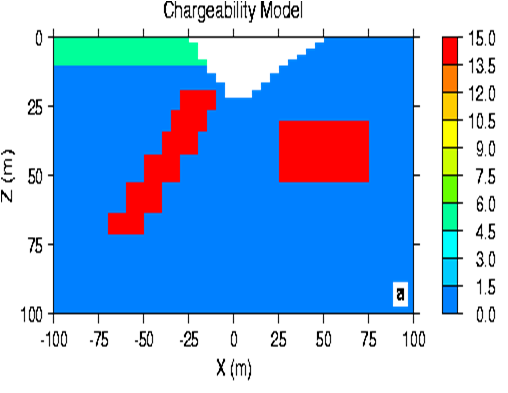
\includegraphics[width=0.5\columnwidth]{fwdTrueCharge}} \\ 
\subfloat[][]{\label{fig:fwdAppCharge}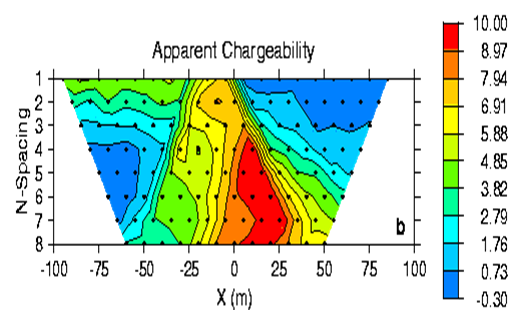
\includegraphics[width=0.5\columnwidth]{fwdAppCharge}}
\caption{(a) The chargeability model associated with the conductivity (Figure \ref{fig:fwdTrueCrop}). (b) The apparent chargeability pseudo-section measured using a pole-dipole array with $a=10$ m and $n=1,8$. The data have been contaminated by Gaussian noise.}
\end{figure}
%
